\documentclass{standalone}
\usepackage{tikz}
\usepackage{ctex,siunitx}
\usepackage{tkz-euclide}
\usepackage{amsmath}
\usetikzlibrary{patterns, calc}
\usetikzlibrary {decorations.pathmorphing, decorations.pathreplacing, decorations.shapes,}
\begin{document}
\small
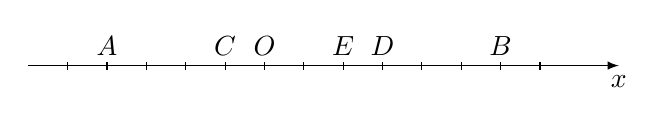
\begin{tikzpicture}[>=latex]
\draw[->](-3,0)--(4.5,0)node[below]{$x$};
\foreach \x in {-2.5,-2,...,3.5}
{
  \draw[thin](\x,-0.05)--++(0,0.1);
}
\node at (0,0)[above]{$O$};
\node at (3,0)[above]{$B$};
\node at (-2,0)[above]{$A$};
\node at (-0.5,0)[above]{$C$};
\node at (1.5,0)[above]{$D$};
\node at (1,0)[above]{$E$};
% \fill (1.6,0)circle(1pt)node[above]{$P$};
\end{tikzpicture}
\end{document}